\documentclass{ximera}


\graphicspath{
  {./}
  {ximeraTutorial/}
  {basicPhilosophy/}
}

\newcommand{\mooculus}{\textsf{\textbf{MOOC}\textnormal{\textsf{ULUS}}}}

\usepackage{tkz-euclide}\usepackage{tikz}
\usepackage{tikz-cd}
\usetikzlibrary{arrows}
\tikzset{>=stealth,commutative diagrams/.cd,
  arrow style=tikz,diagrams={>=stealth}} %% cool arrow head
\tikzset{shorten <>/.style={ shorten >=#1, shorten <=#1 } } %% allows shorter vectors

\usetikzlibrary{backgrounds} %% for boxes around graphs
\usetikzlibrary{shapes,positioning}  %% Clouds and stars
\usetikzlibrary{matrix} %% for matrix
\usepgfplotslibrary{polar} %% for polar plots
\usepgfplotslibrary{fillbetween} %% to shade area between curves in TikZ
\usetkzobj{all}
\usepackage[makeroom]{cancel} %% for strike outs
%\usepackage{mathtools} %% for pretty underbrace % Breaks Ximera
%\usepackage{multicol}
\usepackage{pgffor} %% required for integral for loops



%% http://tex.stackexchange.com/questions/66490/drawing-a-tikz-arc-specifying-the-center
%% Draws beach ball
\tikzset{pics/carc/.style args={#1:#2:#3}{code={\draw[pic actions] (#1:#3) arc(#1:#2:#3);}}}



\usepackage{array}
\setlength{\extrarowheight}{+.1cm}
\newdimen\digitwidth
\settowidth\digitwidth{9}
\def\divrule#1#2{
\noalign{\moveright#1\digitwidth
\vbox{\hrule width#2\digitwidth}}}






\DeclareMathOperator{\arccot}{arccot}
\DeclareMathOperator{\arcsec}{arcsec}
\DeclareMathOperator{\arccsc}{arccsc}

















%%This is to help with formatting on future title pages.
\newenvironment{sectionOutcomes}{}{}



\author{Lee Wayand}

\begin{document}










\begin{exercise}


This is a \textbf{map representation} of the \textit{ShirtPresents} function. \\

Arrows point from the domain to the codomain and indicate a pairing in the function.

\begin{image}
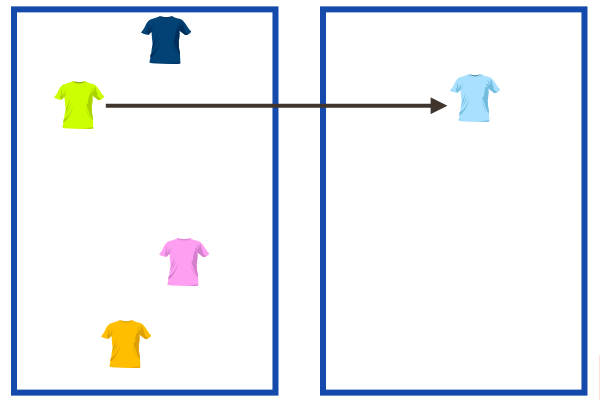
\includegraphics{pics/f_11.png}
\end{image}



Select all of the members of the preimage of \huge\{ \includegraphics{pics/boyHeadphones.png} \huge\}



\begin{selectAll}
\choice [correct]{\includegraphics{pics/lightGreenShirt.png}}
\choice {\includegraphics{pics/lightBlueShirt.png}}
\choice {\includegraphics{pics/orangeShirt.png}}
\choice [correct]{\includegraphics{pics/darkBlueShirt.png}}
\choice {\includegraphics{pics/purpleShirt.png}}
\choice {\includegraphics{pics/redShirt.png}}
\choice {\includegraphics{pics/pinkShirt.png}}
\choice {Cannot be Determined}
\end{selectAll}



\end{exercise}















\begin{exercise}


This is a \textbf{map representation} of the \textit{ShirtPresents} function. \\

Arrows point from the domain to the codomain and indicate a pairing in the function.

\begin{image}
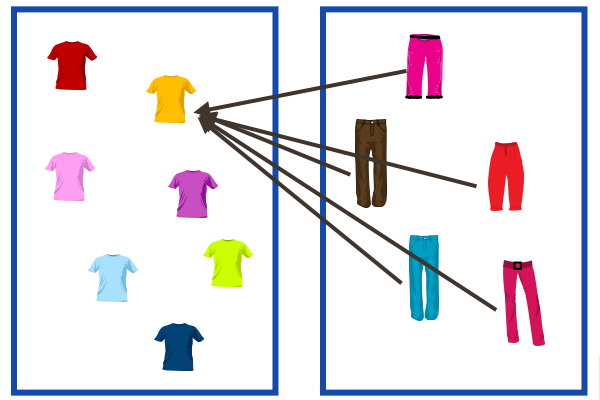
\includegraphics{pics/f_17.png}
\end{image}



Select all of the members of $f^{-1}$\huge( \huge\{ \includegraphics{pics/lightBlueShirt.png}, \includegraphics{pics/darkBlueShirt.png} \huge\} \huge)



\begin{selectAll}
\choice [correct]{\includegraphics{pics/lightGreenShirt.png}}
\choice {\includegraphics{pics/orangeShirt.png}}
\choice [correct]{\includegraphics{pics/darkBlueShirt.png}}
\choice {\includegraphics{pics/redShirt.png}}
\choice [correct]{\includegraphics{pics/pinkShirt.png}}
\choice {Cannot be Determined}
\end{selectAll}



\end{exercise}












\end{document}